\documentclass[aspectratio=169,11pt]{beamer}

% Theme and colors
\usetheme{Madrid}
\usecolortheme{whale}
\setbeamertemplate{navigation symbols}{}
\setbeamertemplate{footline}[frame number]

% Packages
\usepackage[utf8]{inputenc}
\usepackage[T1]{fontenc}
\usepackage{graphicx}
\usepackage{booktabs}
\usepackage{amsmath}
\usepackage{hyperref}
\usepackage{tikz}
\usetikzlibrary{shapes,arrows,positioning,calc,fit,backgrounds,decorations.pathmorphing,patterns}
\usepackage{siunitx}
\usepackage{xcolor}

% Custom colors
\definecolor{questionbg}{RGB}{255,248,220}
\definecolor{questionborder}{RGB}{255,193,7}

% Title information
\title[EECE5155 -- Module 6]{Data Streaming Protocols for IoT}
\subtitle{Module 6: From Device to Cloud}
\author{Eduardo Baena}
\date{Spring 2026}
\institute{Northeastern University\\Department of Electrical and Computer Engineering\\
\texttt{e.baena@northeastern.edu}}

\begin{document}

% Title slide
\begin{frame}
    \titlepage
    \vspace{-1cm}
    \begin{center}
        \textbf{EECE5155: Wireless Sensor Networks and the Internet of Things}
    \end{center}
\end{frame}

% Learning Objectives
\begin{frame}{Learning Objectives}
    \textbf{By the end of this module, you should be able to:}
    
    \vspace{0.5cm}
    \begin{enumerate}
        \item \textbf{Explain} the role of application-layer data streaming in the IoT pipeline
        \item \textbf{Compare} MQTT, CoAP, HTTP, AMQP, and XMPP at the protocol level
        \item \textbf{Design} a publish/subscribe architecture using MQTT 5.0
        \item \textbf{Select} the appropriate streaming protocol for a given IoT scenario
        \item \textbf{Evaluate} emerging approaches: MQTT over QUIC, Sparkplug B, Unified Namespace
    \end{enumerate}
    
    \vspace{0.3cm}
    \begin{alertblock}{Context}
        We have covered how data is acquired (Mod.\ 1--2), processed locally (Mod.\ 3), and transmitted wirelessly (Mod.\ 4--5). Now: how does data flow from device to cloud application?
    \end{alertblock}
\end{frame}

% Outline
\begin{frame}{Outline}
    \begin{columns}
        \column{0.5\textwidth}
        \begin{enumerate}
            \item \textbf{Why Data Streaming?}
            \begin{itemize}
                \item The application-layer problem
                \item Request/response vs publish/subscribe
            \end{itemize}
            
            \item \textbf{MQTT}
            \begin{itemize}
                \item Pub/sub model, topics, QoS
                \item MQTT 5.0 new features
                \item Sparkplug B and Unified Namespace
                \item MQTT over QUIC
            \end{itemize}
            
            \item \textbf{HTTP for IoT}
            \begin{itemize}
                \item REST APIs and methods
                \item HTTP/1.1 $\rightarrow$ HTTP/2 $\rightarrow$ HTTP/3 (QUIC)
            \end{itemize}
        \end{enumerate}
        
        \column{0.5\textwidth}
        \begin{enumerate}
            \setcounter{enumi}{3}
            \item \textbf{CoAP}
            \begin{itemize}
                \item Constrained REST over UDP
                \item Observe pattern
                \item LwM2M device management
            \end{itemize}
            
            \item \textbf{XMPP and AMQP}
            \begin{itemize}
                \item When they make sense
            \end{itemize}
            
            \item \textbf{Emerging Approaches}
            \begin{itemize}
                \item WebSocket, gRPC
                \item Edge streaming architectures
            \end{itemize}
            
            \item \textbf{Protocol Selection Guide}
        \end{enumerate}
    \end{columns}
\end{frame}

%==============================================================================
\section{Why Data Streaming?}
%==============================================================================

\begin{frame}{The Application-Layer Problem}
    \textbf{You have data at the edge. How do you get it to the cloud (and back)?}
    
    \vspace{0.2cm}
    \begin{columns}
        \column{0.5\textwidth}
        \textbf{Why not just use FTP or email?}
        \begin{itemize}
            \item \textbf{FTP/SFTP:} File transfer, too heavy
            \item \textbf{SMTP/IMAP:} Email, absurd overhead for 20-byte payloads
            \item \textbf{Raw TCP sockets:} No structure, no interop
        \end{itemize}
        
        \vspace{0.15cm}
        \textbf{IoT needs:}
        \begin{itemize}
            \item Small messages, frequently
            \item Low overhead (bandwidth, memory)
            \item Reliability options (QoS)
            \item Security (authentication, encryption)
            \item Scalability (thousands of devices)
        \end{itemize}
        
        \column{0.5\textwidth}
        \textbf{Two fundamental patterns:}
        
        \vspace{0.15cm}
        \begin{center}
        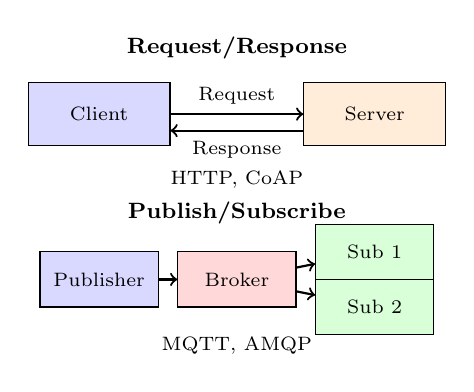
\begin{tikzpicture}[scale=0.7, every node/.style={font=\scriptsize}]
            % Request/Response
            \node[draw, fill=blue!15, minimum width=1.8cm, minimum height=0.8cm] (client) at (0,3) {Client};
            \node[draw, fill=orange!15, minimum width=1.8cm, minimum height=0.8cm] (server) at (5,3) {Server};
            \draw[->, thick] (client.east) -- node[above]{Request} (server.west);
            \draw[<-, thick] ([yshift=-3mm]client.east) -- node[below]{Response} ([yshift=-3mm]server.west);
            \node[font=\footnotesize\bfseries] at (2.5,4.2) {Request/Response};
            \node at (2.5,1.8) {HTTP, CoAP};
            
            % Pub/Sub
            \node[draw, fill=blue!15, minimum width=1.5cm, minimum height=0.7cm] (pub) at (0,0) {Publisher};
            \node[draw, fill=red!15, minimum width=1.5cm, minimum height=0.7cm] (broker) at (2.5,0) {Broker};
            \node[draw, fill=green!15, minimum width=1.5cm, minimum height=0.7cm] (sub1) at (5,0.5) {Sub 1};
            \node[draw, fill=green!15, minimum width=1.5cm, minimum height=0.7cm] (sub2) at (5,-0.5) {Sub 2};
            \draw[->, thick] (pub) -- (broker);
            \draw[->, thick] (broker) -- (sub1);
            \draw[->, thick] (broker) -- (sub2);
            \node[font=\footnotesize\bfseries] at (2.5,1.2) {Publish/Subscribe};
            \node at (2.5,-1.2) {MQTT, AMQP};
        \end{tikzpicture}
        \end{center}
    \end{columns}
\end{frame}

%==============================================================================
\section{MQTT}
%==============================================================================

\begin{frame}{MQTT: Message Queuing Telemetry Transport}
    \begin{columns}
        \column{0.5\textwidth}
        \textbf{Origin:}
        \begin{itemize}
            \item Invented 1999 by Andy Stanford-Clark (IBM) and Arlen Nipper
            \item Original use: oil pipeline sensors via satellite
            \item OASIS standard: MQTT 3.1.1 (2014)
            \item ISO/IEC 20922 (2016)
            \item \textbf{MQTT 5.0} (2019) --- current version
        \end{itemize}
        
        \vspace{0.2cm}
        \textbf{Properties:}
        \begin{itemize}
            \item Publish/subscribe over \textbf{TCP/IP}
            \item Small code footprint ($\sim$kB)
            \item 2-byte minimum header
            \item Up to 256 MB payload (usually much less)
            \item Designed for low bandwidth, high latency
        \end{itemize}
        
        \column{0.5\textwidth}
        \textbf{Who uses MQTT (2025)?}
        \begin{itemize}
            \item AWS IoT Core
            \item Azure IoT Hub
            \item Google Cloud IoT
            \item Facebook Messenger (billions of msgs/day)
            \item LoRaWAN gateways (The Things Network)
            \item Tesla, BMW (connected vehicles)
            \item Siemens, Bosch (industrial IoT)
        \end{itemize}
        
        \vspace{0.2cm}
        \begin{exampleblock}{Why MQTT Dominates IoT}
            Lightweight + QoS options + widespread broker/cloud support = \textbf{de facto standard} for device-to-cloud telemetry.
        \end{exampleblock}
    \end{columns}
\end{frame}

\begin{frame}{MQTT Publish/Subscribe Model}
    \begin{columns}
        \column{0.55\textwidth}
        \textbf{Core architecture:}
        \begin{itemize}
            \item \textbf{Publisher:} device that sends data to a \textit{topic}
            \item \textbf{Broker:} central server that receives and routes messages
            \item \textbf{Subscriber:} client that receives messages on subscribed topics
            \item Publishers and subscribers are \textbf{decoupled} --- they never communicate directly
        \end{itemize}
        
        \vspace{0.2cm}
        \textbf{Topic structure} (hierarchical, like file paths):
        \begin{itemize}
            \item \texttt{vineyard/zone1/soil/moisture}
            \item \texttt{vineyard/zone1/weather/temperature}
            \item \texttt{factory/line3/pump7/vibration}
        \end{itemize}
        
        \column{0.45\textwidth}
        \textbf{Wildcards for subscriptions:}
        \begin{itemize}
            \item \texttt{+} single level: \texttt{vineyard/+/soil/\#}
            \item \texttt{\#} multi-level: \texttt{vineyard/\#} (all under vineyard)
        \end{itemize}
        
        \vspace{0.2cm}
        \begin{alertblock}{Key Advantage}
            Adding a new subscriber requires \textbf{zero changes} to publishers. Adding a new publisher requires \textbf{zero changes} to subscribers.
            
            \vspace{0.1cm}
            This decoupling is why pub/sub scales better than request/response for IoT.
        \end{alertblock}
    \end{columns}
\end{frame}

\begin{frame}{MQTT Protocol: Session Lifecycle}
    \textbf{An MQTT session has four stages:}
    
    \vspace{0.2cm}
    \begin{enumerate}
        \item \textbf{Connection:} \texttt{CONNECT} / \texttt{CONNACK}
        \begin{itemize}
            \item Client opens TCP to broker (port 1883, or 8883 for TLS)
            \item Sends client ID, optional username/password, keep-alive interval
            \item \textbf{Will message:} if client disconnects unexpectedly, broker publishes this to a specified topic (``last will and testament'')
        \end{itemize}
        
        \item \textbf{Authentication:}
        \begin{itemize}
            \item Without TLS: username/password in \textbf{clear text} (insecure!)
            \item With TLS: server certificate validation; optional mutual TLS (client cert)
        \end{itemize}
        
        \item \textbf{Communication:}
        \begin{itemize}
            \item \texttt{PUBLISH}, \texttt{SUBSCRIBE} / \texttt{SUBACK}, \texttt{UNSUBSCRIBE} / \texttt{UNSUBACK}
            \item \texttt{PINGREQ} / \texttt{PINGRESP} to keep TCP alive
        \end{itemize}
        
        \item \textbf{Termination:} \texttt{DISCONNECT}
    \end{enumerate}
\end{frame}

\begin{frame}{MQTT Quality of Service (QoS)}
    \textbf{Three delivery guarantees:}
    
    \vspace{0.15cm}
    \begin{center}
    \footnotesize
    \begin{tabular}{clp{4.5cm}c}
        \toprule
        \textbf{QoS} & \textbf{Guarantee} & \textbf{Messages} & \textbf{Overhead} \\
        \midrule
        0 & At most once & PUBLISH & Low \\
        1 & At least once & PUBLISH / PUBACK & Medium \\
        2 & Exactly once & PUBLISH / PUBREC / PUBREL / PUBCOMP & High \\
        \bottomrule
    \end{tabular}
    \normalsize
    \end{center}
    
    \vspace{0.1cm}
    \begin{columns}
        \column{0.33\textwidth}
        \textbf{QoS 0:}
        \begin{itemize}
            \item No ACK, no retry
            \item For high-frequency telemetry
        \end{itemize}
        
        \column{0.33\textwidth}
        \textbf{QoS 1:}
        \begin{itemize}
            \item ACK per message
            \item May deliver duplicates
        \end{itemize}
        
        \column{0.33\textwidth}
        \textbf{QoS 2:}
        \begin{itemize}
            \item 4-packet handshake
            \item No duplicates, no loss
        \end{itemize}
    \end{columns}
    
    \begin{alertblock}{Design Decision}
        QoS 2 costs 4x the messages of QoS 0. For soil sensors, QoS 1 is the right balance.
    \end{alertblock}
\end{frame}

\begin{frame}{MQTT Challenges}
    \begin{columns}
        \column{0.5\textwidth}
        \textbf{Scalability:}
        \begin{itemize}
            \item Topic tree can grow enormous
            \item No built-in federation between brokers
            \item Hard to partition topic namespace across clusters
        \end{itemize}
        
        \vspace{0.2cm}
        \textbf{Interoperability:}
        \begin{itemize}
            \item Payload is \textbf{opaque binary}
            \item No defined encoding (JSON? Protobuf? CBOR?)
            \item Different manufacturers $\Rightarrow$ incompatible payloads
        \end{itemize}
        
        \column{0.5\textwidth}
        \textbf{Security:}
        \begin{itemize}
            \item Minimal built-in auth (username/password)
            \item Any real security requires \textbf{TLS}
            \item TLS adds latency and memory overhead
            \item Challenge on constrained MCUs ($<$64 kB RAM)
        \end{itemize}
        
        \vspace{0.2cm}
        \textbf{Transport:}
        \begin{itemize}
            \item TCP-based: connection overhead
            \item Head-of-line blocking
            \item Slow reconnection after network change
        \end{itemize}
        
        \vspace{0.1cm}
        \begin{exampleblock}{MQTT 5.0 addresses many of these}
            See next slides...
        \end{exampleblock}
    \end{columns}
\end{frame}

\begin{frame}{MQTT 5.0 (2019): Key New Features}
    \textbf{MQTT 5.0 adds 7 major features over 3.1.1:}
    
    \vspace{0.2cm}
    \footnotesize
    \begin{center}
    \begin{tabular}{p{3.5cm}p{4.5cm}p{4cm}}
        \toprule
        \textbf{Feature} & \textbf{What It Does} & \textbf{Why It Matters for IoT} \\
        \midrule
        \textbf{Reason Codes} & Every ACK includes a code explaining success/failure & Better diagnostics on constrained devices \\
        \addlinespace
        \textbf{Session Expiry} & Client specifies how long broker keeps session after disconnect & Saves broker memory; configurable per device \\
        \addlinespace
        \textbf{Topic Aliases} & Short numeric alias replaces long topic string & Reduces header size on repeated publishes \\
        \addlinespace
        \textbf{User Properties} & Custom key-value metadata in packet headers & Timestamps, device location, data encoding \\
        \addlinespace
        \textbf{Subscription Options} & Per-topic control over retained msgs, QoS behavior & Finer-grained subscription management \\
        \addlinespace
        \textbf{Request/Response} & Client specifies reply-to topic in PUBLISH & Enables RPC-like patterns over MQTT \\
        \addlinespace
        \textbf{Shared Subscriptions} & Multiple subscribers load-balance a topic & Horizontal scaling of backend consumers \\
        \bottomrule
    \end{tabular}
    \end{center}
    \normalsize
    
    \vspace{0.1cm}
    \begin{alertblock}{Adoption Status (2025)}
        All major brokers support MQTT 5.0: EMQX, Mosquitto 2.x, HiveMQ, AWS IoT Core.
    \end{alertblock}
\end{frame}

\begin{frame}{MQTT Sparkplug B: Solving the Payload Problem}
    \textbf{Problem:} MQTT defines \textit{how} to send messages, but not \textit{what} they contain.
    
    \vspace{0.2cm}
    \begin{columns}
        \column{0.5\textwidth}
        \textbf{Sparkplug B} (Eclipse Foundation, OASIS standard):
        \begin{itemize}
            \item Standardized \textbf{topic namespace}:\\
            \texttt{spBv1.0/group/DDATA/node/device}
            \item Standardized \textbf{payload format} (Protobuf-encoded)
            \item \textbf{Birth/Death certificates:}
            \begin{itemize}
                \item NBIRTH: node comes online with full metric list
                \item NDEATH: node goes offline (via MQTT will message)
                \item State is always known!
            \end{itemize}
            \item Report by exception (only changed values)
            \item Automatic metric discovery
        \end{itemize}
        
        \column{0.5\textwidth}
        \textbf{Unified Namespace (UNS):}
        \begin{itemize}
            \item Architecture pattern using MQTT + Sparkplug
            \item \textbf{Single source of truth} for all industrial data
            \item Replaces point-to-point integrations (OPC-UA, Modbus, proprietary APIs)
            \item Any system can publish/subscribe to the same broker
        \end{itemize}
        
        \vspace{0.1cm}
        \begin{exampleblock}{Industry 4.0 Trend (2024--2025)}
            UNS is the dominant architecture pattern for smart manufacturing. Siemens, Bosch, BMW use Sparkplug B + MQTT to unify IT and OT data.
        \end{exampleblock}
    \end{columns}
\end{frame}

\begin{frame}{MQTT over QUIC: Beyond TCP}
    \textbf{Problem:} MQTT runs on TCP, which has inherent limitations:
    \begin{itemize}
        \item Slow reconnection after network handoff (e.g., vehicle entering tunnel)
        \item Head-of-line blocking: one lost packet stalls all messages
        \item TLS handshake adds latency (1--2 RTT)
    \end{itemize}
    
    \vspace{0.15cm}
    \textbf{Solution: MQTT over QUIC} (EMQX 5.0, 2023):
    
    \begin{columns}
        \column{0.5\textwidth}
        \begin{itemize}
            \item \textbf{0-RTT reconnection:} resume session instantly
            \item \textbf{Connection migration:} seamless IP change (Wi-Fi $\rightarrow$ cellular)
            \item \textbf{No head-of-line blocking:} independent streams
            \item \textbf{Built-in TLS 1.3:} security with no extra handshake
        \end{itemize}
        
        \column{0.5\textwidth}
        \begin{center}
        \begin{tabular}{lcc}
            \toprule
            & \textbf{TCP/TLS} & \textbf{QUIC} \\
            \midrule
            New conn. & 3 RTT & 1 RTT \\
            Reconnect & 2 RTT & \textbf{0 RTT} \\
            IP change & Reconnect & \textbf{Migrate} \\
            Encryption & TLS 1.2/1.3 & TLS 1.3 \\
            \bottomrule
        \end{tabular}
        \end{center}
        
        \begin{alertblock}{Status (2026)}
            EMQX supports MQTT over QUIC natively. IETF standardization in progress.
        \end{alertblock}
    \end{columns}
\end{frame}

%==============================================================================
\section{HTTP for IoT}
%==============================================================================

\begin{frame}{HTTP: The Universal Protocol}
    \textbf{HTTP is old (RFC 2616, 1999) but still valid for IoT because:}
    
    \vspace{0.2cm}
    \begin{columns}
        \column{0.5\textwidth}
        \textbf{Advantages:}
        \begin{itemize}
            \item Most compatible with existing infrastructure
            \item If a web browser works, HTTP will work
            \item Stateless: traverses firewalls and NAT easily
            \item Well-understood auth (OAuth2, API keys, JWT)
            \item Mature TLS support
            \item REST APIs are universal
        \end{itemize}
        
        \vspace{0.2cm}
        \textbf{Disadvantages for IoT:}
        \begin{itemize}
            \item Large headers (hundreds of bytes)
            \item Request/response only (no push by default)
            \item High memory footprint for TLS
            \item TCP connection overhead
        \end{itemize}
        
        \column{0.5\textwidth}
        \textbf{HTTP Methods for IoT REST APIs:}
        \begin{center}
        \begin{tabular}{ll}
            \toprule
            \textbf{Method} & \textbf{IoT Use} \\
            \midrule
            \texttt{GET} & Read sensor value \\
            \texttt{POST} & Submit new reading \\
            \texttt{PUT} & Update device config \\
            \texttt{DELETE} & Remove device \\
            \bottomrule
        \end{tabular}
        \end{center}
        
        \vspace{0.2cm}
        \textbf{When to use HTTP for IoT:}
        \begin{itemize}
            \item Gateway-to-cloud (not device-to-cloud)
            \item Infrequent, large payloads
            \item Integration with web services
            \item Mains-powered devices
        \end{itemize}
    \end{columns}
\end{frame}

\begin{frame}{HTTP Evolution: From 1.0 to HTTP/3}
    \begin{center}
    \begin{tabular}{lcccc}
        \toprule
        & \textbf{HTTP/1.0} & \textbf{HTTP/1.1} & \textbf{HTTP/2} & \textbf{HTTP/3} \\
        \midrule
        Year & 1996 & 1997 & 2015 & \textbf{2022 (RFC 9114)} \\
        Transport & TCP & TCP (persistent) & TCP & \textbf{QUIC (UDP)} \\
        Connections & 1 req/conn & Pipelined & Multiplexed & Multiplexed \\
        Header & Text & Text & \textbf{Binary, HPACK} & \textbf{Binary, QPACK} \\
        Server push & No & No & Yes & Yes \\
        HoL blocking & Yes & Yes & TCP-level & \textbf{No} \\
        TLS & Optional & Optional & Effectively req. & \textbf{Built-in 1.3} \\
        \bottomrule
    \end{tabular}
    \end{center}
    
    \vspace{0.1cm}
    \begin{columns}
        \column{0.5\textwidth}
        \begin{exampleblock}{HTTP/3 for IoT (2025)}
            QUIC transport eliminates head-of-line blocking and enables 0-RTT reconnection. Research shows HTTP/3 pub/sub can rival MQTT for constrained IoT.
        \end{exampleblock}
        
        \column{0.5\textwidth}
        \begin{alertblock}{Adoption Status}
            30\%+ of web traffic uses HTTP/3 (Cloudflare, Google). IoT adoption still early: most MCU HTTP stacks support 1.1 only. Gateways can bridge to HTTP/3.
        \end{alertblock}
    \end{columns}
\end{frame}

%==============================================================================
\section{CoAP}
%==============================================================================

\begin{frame}{CoAP: Constrained Application Protocol}
    \textbf{RFC 7252 (2014), IETF CoRE working group.}
    
    \vspace{0.05cm}
    \begin{columns}
        \column{0.5\textwidth}
        \textbf{Design philosophy:} ``HTTP for constrained devices''
        \begin{itemize}
            \item Runs over \textbf{UDP} (not TCP!)
            \item 4-byte fixed header (vs hundreds for HTTP)
            \item Max payload: 1024 bytes
            \item Same methods: \texttt{GET}, \texttt{PUT}, \texttt{POST}, \texttt{DELETE}
            \item URIs like HTTP: \texttt{coap://sensor.local/temp}
        \end{itemize}
        
        \vspace{0.05cm}
        \textbf{Message types:}
        \begin{itemize}
            \item \textbf{CON}: retransmit until ACK
            \item \textbf{NON}: fire and forget
            \item \textbf{ACK}: Acknowledgement
            \item \textbf{RST}: cannot process
        \end{itemize}
        
        \column{0.5\textwidth}
        \textbf{Request/Response model:}
        
        \vspace{0.05cm}
        \textit{Piggyback response} (fast):
        \begin{center}
        \scriptsize
        Client $\xrightarrow{\text{CON GET /temp}}$ Server\\
        Client $\xleftarrow{\text{ACK 2.05 [22.5°C]}}$ Server
        \normalsize
        \end{center}
        
        \vspace{0.05cm}
        \textit{Separate response} (slow):
        \begin{center}
        \scriptsize
        Client $\xrightarrow{\text{CON GET /temp}}$ Server\\
        Client $\xleftarrow{\text{ACK (empty)}}$ Server\\
        $\cdots$ server processing $\cdots$\\
        Client $\xleftarrow{\text{CON 2.05 [22.5°C]}}$ Server\\
        Client $\xrightarrow{\text{ACK}}$ Server
        \normalsize
        \end{center}
        
        \begin{alertblock}{Key Advantage}
            UDP = no connection state, no handshake. Ideal for battery-powered sensors.
        \end{alertblock}
    \end{columns}
\end{frame}

\begin{frame}{CoAP Observe and LwM2M}
    \begin{columns}
        \column{0.5\textwidth}
        \textbf{CoAP Observe} (RFC 7641):
        \begin{itemize}
            \item Adds \textbf{publish/subscribe} to CoAP
            \item Client sends GET with Observe option
            \item Server sends notifications on resource change
            \item Like MQTT subscribe, but peer-to-peer (no broker)
        \end{itemize}
        
        \vspace{0.3cm}
        \textbf{CoAP vs MQTT:}
        \begin{center}
        \footnotesize
        \begin{tabular}{lcc}
            \toprule
            & \textbf{CoAP} & \textbf{MQTT} \\
            \midrule
            Transport & UDP & TCP \\
            Pattern & RESTful & Pub/sub \\
            Broker & No & Yes (required) \\
            Header & 4 bytes & 2 bytes \\
            Multicast & Yes & No \\
            Observe & Optional & Native \\
            \bottomrule
        \end{tabular}
        \normalsize
        \end{center}
        
        \column{0.5\textwidth}
        \textbf{OMA LwM2M} (Lightweight M2M):
        \begin{itemize}
            \item \textbf{Device management protocol} built on CoAP
            \item OMA SpecWorks standard (v1.0: 2017, \textbf{v1.2: 2022})
            \item Defines standardized \textbf{object model}:
            \begin{itemize}
                \item Object 3: Device (manufacturer, model, battery)
                \item Object 3303: Temperature sensor
                \item Object 3304: Humidity sensor
                \item 200+ registered objects
            \end{itemize}
            \item Operations: Read, Write, Execute, Observe
            \item Bootstrap + Registration + Firmware update
        \end{itemize}
        
        \vspace{0.1cm}
        \begin{exampleblock}{LwM2M v1.2 (2022)}
            Added MQTT and HTTP transports (not just CoAP), CBOR data format, gateway support.
        \end{exampleblock}
    \end{columns}
\end{frame}

%==============================================================================
\section{XMPP and AMQP}
%==============================================================================

\begin{frame}{XMPP: Extensible Messaging and Presence Protocol}
    \begin{columns}
        \column{0.5\textwidth}
        \textbf{Origin:} Jabber instant messaging (1999), IETF standard (RFC 6120/6121).
        
        \vspace{0.2cm}
        \textbf{Key features:}
        \begin{itemize}
            \item XML-based messaging
            \item JID addressing: \texttt{user@domain/resource}
            \item Three stanza types: \texttt{message}, \texttt{presence}, \texttt{iq} (info/query)
            \item Decentralized (federated servers)
            \item Rich service discovery
            \item Extensible via XEPs (XMPP Extension Protocols)
        \end{itemize}
        
        \vspace{0.2cm}
        \textbf{IoT extensions (XEP-0323/0325):}
        \begin{itemize}
            \item Sensor data reading and control
            \item Provisioning and discovery
        \end{itemize}
        
        \column{0.5\textwidth}
        \textbf{Drawbacks for constrained IoT:}
        \begin{itemize}
            \item \textbf{XML is heavy:} verbose text format
            \item XML parser needs significant RAM ($>$64 kB)
            \item Presence messages = high overhead for many devices
            \item Designed for human IM, not machine telemetry
        \end{itemize}
        
        \vspace{0.1cm}
        \begin{alertblock}{Verdict (2025)}
            XMPP is well-suited for \textbf{chat-like IoT} (smart home UIs) but \textbf{not for constrained sensors}. Its niche has been absorbed by MQTT + WebSocket.
        \end{alertblock}
    \end{columns}
\end{frame}

\begin{frame}{AMQP: Advanced Message Queuing Protocol}
    \begin{columns}
        \column{0.5\textwidth}
        \textbf{Origin:} Financial services (JPMorgan, 2003). OASIS standard, ISO/IEC 19464.
        
        \vspace{0.2cm}
        \textbf{Key features:}
        \begin{itemize}
            \item Binary wire protocol (efficient)
            \item Peer-to-peer OR broker-mediated
            \item \textbf{Credit-based flow control:} receiver controls message rate
            \item Rich message semantics:
            \begin{itemize}
                \item Links, sessions, connections (layered)
                \item Transactions and settlements
                \item Multiple message disposition states
            \end{itemize}
            \item Runs over TCP
        \end{itemize}
        
        \column{0.5\textwidth}
        \textbf{AMQP Frame Types:}
        \begin{enumerate}
            \item \texttt{open} / \texttt{close} (connection)
            \item \texttt{begin} / \texttt{end} (session)
            \item \texttt{attach} / \texttt{detach} (link)
            \item \texttt{transfer} (data)
            \item \texttt{flow} (credit control)
            \item \texttt{disposition} (settlement)
        \end{enumerate}
        
        \vspace{0.1cm}
        \begin{alertblock}{AMQP vs MQTT}
            AMQP is \textbf{more powerful} but \textbf{much heavier}. Use AMQP for backend/cloud routing (RabbitMQ, Azure Service Bus). Use MQTT for device-to-broker edge.
        \end{alertblock}
    \end{columns}
\end{frame}

%==============================================================================
\section{Emerging Approaches}
%==============================================================================

\begin{frame}{WebSocket, gRPC, and Edge Streaming}
    \begin{columns}
        \column{0.5\textwidth}
        \textbf{WebSocket} (RFC 6455, 2011):
        \begin{itemize}
            \item Full-duplex over a single TCP connection
            \item Starts as HTTP upgrade, then raw frames
            \item Low overhead after handshake (2--14 byte header)
            \item Browser-native (JavaScript API)
            \item Use case: real-time dashboards, MQTT over WebSocket (browser $\leftrightarrow$ broker)
        \end{itemize}
        
        \vspace{0.2cm}
        \textbf{gRPC} (Google, 2015):
        \begin{itemize}
            \item RPC framework over HTTP/2
            \item Protobuf serialization (compact binary)
            \item Bidirectional streaming
            \item Strong typing via \texttt{.proto} files
            \item Use case: edge$\leftrightarrow$cloud microservices, not constrained devices
        \end{itemize}
        
        \column{0.5\textwidth}
        \textbf{Edge Streaming Architectures (2024--2025):}
        
        \vspace{0.2cm}
        \begin{center}
        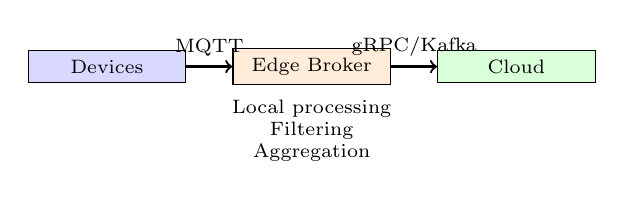
\begin{tikzpicture}[scale=0.65, every node/.style={font=\scriptsize}]
            \node[draw, fill=blue!15, minimum width=2cm] (dev) at (0,0) {Devices};
            \node[draw, fill=orange!15, minimum width=2cm] (edge) at (4,0) {Edge Broker};
            \node[draw, fill=green!15, minimum width=2cm] (cloud) at (8,0) {Cloud};
            \draw[->, thick] (dev) -- node[above]{MQTT} (edge);
            \draw[->, thick] (edge) -- node[above]{gRPC/Kafka} (cloud);
            \node[below=0.3cm, align=center] at (edge) {Local processing\\Filtering\\Aggregation};
        \end{tikzpicture}
        \end{center}
        
        \vspace{0.2cm}
        \textbf{Apache Kafka for IoT:}
        \begin{itemize}
            \item Distributed event log (not broker)
            \item Massive throughput ($>$1M msgs/s)
            \item Persistent, replayable streams
            \item Not for constrained devices---for \textbf{cloud-side} ingestion
            \item Pattern: MQTT $\rightarrow$ edge $\rightarrow$ Kafka $\rightarrow$ analytics
        \end{itemize}
    \end{columns}
\end{frame}

%==============================================================================
\section{Protocol Selection}
%==============================================================================

\begin{frame}{Protocol Comparison: Head-to-Head}
    \footnotesize
    \begin{center}
    \begin{tabular}{lccccc}
        \toprule
        & \textbf{MQTT 5.0} & \textbf{CoAP} & \textbf{HTTP/1.1} & \textbf{AMQP} & \textbf{XMPP} \\
        \midrule
        Transport & TCP & \textbf{UDP} & TCP & TCP & TCP \\
        Pattern & Pub/sub & Request/resp & Request/resp & Pub/sub & Presence/IM \\
        Header size & 2 B & 4 B & 100s B & 8 B & XML (large) \\
        Payload fmt & Binary (any) & Binary (any) & Text/binary & Binary & XML \\
        Max payload & 256 MB & 1 kB (typ.) & Unlimited & Unlimited & Unlimited \\
        QoS levels & 0, 1, 2 & CON/NON & TCP only & Settlements & --- \\
        Encryption & TLS & DTLS & TLS & TLS & TLS \\
        Multicast & No & \textbf{Yes} & No & No & No \\
        Broker req. & Yes & No & No & Optional & No \\
        RAM (MCU) & 10--50 kB & \textbf{5--15 kB} & 50--100 kB & 100+ kB & 100+ kB \\
        Std. body & OASIS & IETF & IETF & OASIS/ISO & IETF \\
        \bottomrule
    \end{tabular}
    \end{center}
    \normalsize
\end{frame}

\begin{frame}{Protocol Selection Guide: Think in Constraints}
    \textbf{Use the elimination method} (same as for wireless protocols):
    
    \vspace{0.3cm}
    \begin{center}
    \footnotesize
    \begin{tabular}{p{4.5cm}p{3cm}p{4.5cm}}
        \toprule
        \textbf{If your dominant constraint is...} & \textbf{Choose} & \textbf{Why} \\
        \midrule
        Minimum device RAM ($<$16 kB) & \textbf{CoAP} & Smallest footprint, no TCP stack needed \\
        \addlinespace
        Many devices $\rightarrow$ one cloud & \textbf{MQTT 5.0} & Pub/sub decoupling, shared subscriptions \\
        \addlinespace
        Existing web/REST infrastructure & \textbf{HTTP} & Zero new infrastructure \\
        \addlinespace
        Cloud$\leftrightarrow$cloud message routing & \textbf{AMQP} & Transactions, flow control, routing \\
        \addlinespace
        Real-time browser dashboard & \textbf{MQTT over WS} & MQTT pub/sub + browser compatibility \\
        \addlinespace
        Spotty/mobile network & \textbf{MQTT over QUIC} & 0-RTT reconnect, connection migration \\
        \addlinespace
        Device management + firmware OTA & \textbf{CoAP + LwM2M} & Standardized object model, OMA standard \\
        \addlinespace
        Industrial data unification & \textbf{MQTT + Sparkplug B} & Unified namespace, birth/death certs \\
        \bottomrule
    \end{tabular}
    \normalsize
    \end{center}
    
    \vspace{0.1cm}
    \begin{alertblock}{No ``Best'' Protocol}
        Choose based on your constraints. Many real systems use \textbf{multiple protocols}: CoAP device$\rightarrow$gateway, MQTT gateway$\rightarrow$cloud, gRPC cloud$\rightarrow$analytics.
    \end{alertblock}
\end{frame}

\begin{frame}{State of the Art: IoT Data Streaming in 2026}
    \begin{columns}
        \column{0.5\textwidth}
        \textbf{Established (production-ready):}
        \begin{itemize}
            \item \textbf{MQTT 5.0:} dominant for device-to-cloud. All major clouds support it natively.
            \item \textbf{CoAP + LwM2M 1.2:} standard for cellular IoT device management (NB-IoT/LTE-M).
            \item \textbf{HTTP REST:} universal glue for cloud-side integrations.
            \item \textbf{AMQP 1.0:} enterprise messaging backbone (Azure Service Bus, RabbitMQ).
        \end{itemize}
        
        \column{0.5\textwidth}
        \textbf{Emerging (gaining traction):}
        \begin{itemize}
            \item \textbf{MQTT over QUIC:} EMQX 5.x production-ready. IETF draft progressing. Critical for connected vehicles.
            \item \textbf{Sparkplug B + UNS:} Industry 4.0 standard architecture. Eclipse Foundation stewardship.
            \item \textbf{HTTP/3 pub/sub:} Research showing viability for constrained IoT.
            \item \textbf{Kafka + MQTT bridge:} Standard edge-to-cloud pipeline for high-volume analytics.
        \end{itemize}
    \end{columns}
    
    \vspace{0.1cm}
    \begin{alertblock}{Trend: Protocol Convergence at the Edge}
        The edge gateway is becoming the protocol translator: devices speak CoAP or MQTT, the cloud speaks HTTP/gRPC/Kafka. The ``protocol war'' is resolved by \textbf{not choosing one protocol}.
    \end{alertblock}
\end{frame}

%==============================================================================
\section{Summary}
%==============================================================================

\begin{frame}{Key Takeaways}
    \begin{columns}
        \column{0.5\textwidth}
        \textbf{Core Protocols:}
        \begin{itemize}
            \item \textbf{MQTT:} Pub/sub over TCP. QoS 0/1/2. De facto IoT standard. MQTT 5.0 adds topic aliases, shared subs, request/response.
            \item \textbf{CoAP:} REST over UDP. 4-byte header. Best for constrained MCUs. Observe adds pub/sub.
            \item \textbf{HTTP:} Universal but heavy. Use for gateway-to-cloud, not device-to-cloud.
        \end{itemize}
        
        \column{0.5\textwidth}
        \textbf{What's New (2024--2026):}
        \begin{itemize}
            \item \textbf{MQTT over QUIC:} 0-RTT reconnect for mobile IoT.
            \item \textbf{Sparkplug B:} Standardized payload + state tracking for industrial IoT.
            \item \textbf{LwM2M 1.2:} Device management now supports MQTT and HTTP transports.
            \item \textbf{Edge architecture:} Multi-protocol gateways are the norm.
        \end{itemize}
    \end{columns}
    
    \vspace{0.1cm}
    \begin{alertblock}{The Meta-Lesson}
        The protocol you choose for device$\rightarrow$gateway is often different from gateway$\rightarrow$cloud. \textbf{Design each hop separately}.
    \end{alertblock}
\end{frame}

\begin{frame}{Questions?}
    \begin{center}
        \Huge Questions?
        
        \vspace{1cm}
        \normalsize
        \textbf{Eduardo Baena}\\
        \texttt{e.baena@northeastern.edu}
        
        \vspace{0.5cm}
        \textit{EECE5155: Wireless Sensor Networks and the Internet of Things}\\
        Spring 2026
    \end{center}
\end{frame}

\end{document}
